% Please use the skeleton file you have received in the 
% invitation-to-submit email, where your data are already
% filled in. Otherwise please make sure you insert your 
% data according to the instructions in PoSauthmanual.pdf
\documentclass{PoS}

\title{The $\gamma$-ray Milky Way above 10 GeV:\\
Distinguishing Sources from Diffuse Emission}

\ShortTitle{Distinguishing Sources from Diffuse Emission}

\author{\speaker{E. Owen},$^a$ C. Deil,$^{a}$ A. Donath,$^{a}$ R. Terrier$^{b}$\\
\llap{$^a$}Max-Planck-Institut f\"{u}r Kernphysik, P.O. Box 103980, D
69029 Heidelberg, Germany\\
\llap{$^b$}Astroparticule \& Cosmologie, CNRS, 75205 Paris Cedex 13, France\\
E-mail: \email{ellis.owen@mpi-hd.mpg.de}, \email{christoph.deil@mpi-hd.mpg.de}, \email{axel.donath@mpi-hd.mpg.de}, \email{terrier@apc.univ-paris7.fr}}


\abstract{One of the most prominent features of the $\gamma$-ray sky is the emission from our own galaxy. The Galactic plane has been observed by \textit{Fermi}/LAT in GeV and H.E.S.S. in TeV light. Fermi has modeled the Galactic emission as the sum of a complex "diffuse" emission model with the predominately point source catalogs of 1FHL and 2FGL, while H.E.S.S. has primarily detected extended TeV sources. At GeV energies, Galactic diffuse emission dominates the $\gamma$-ray Milky Way but, as sources have hard spectra, it is likely their emission dominates at TeV energies. Generally the spatial shape and fraction of source emission compared to diffuse emission in the Galactic plane is not well known and is dependent on the source detection method, threshold and diffuse emission modeling methods used. \\

We present a simple image-analysis based method applied to Fermi data from 10 GeV to 500 GeV, covering a region of +/- 5 degrees in Galactic latitude and +/- 100 degrees in Galactic longitude, to separate source and diffuse emission. This method involves significance clipping to exclude sources, combined with elongated filter smoothing. We test the method against models based on the Fermi 1FHL catalog and very simple model Galaxies to evaluate the response for an input of known fraction and shape of diffuse and source emission.}

\FullConference{Science with the New Generation of High Energy Gamma-ray experiments, 10th Workshop - Scineghe2014\\
		04-06 June 2014\\
		Lisbon - Portugal}
    
\usepackage{multirow}
\usepackage{gensymb}
\usepackage{wrapfig}
\usepackage{amsmath}
\usepackage{wasysym}
\begin{document}

\section{Introduction}

In this work, we study methods of separating sources from galactic background emission using image-based techniques at energies above 10 GeV in order to understand appropriate methods for automatic background modelling and source detection.

\subsection{Motivation}

\begin{wrapfigure}{r}{0.5\textwidth}
  \centering
      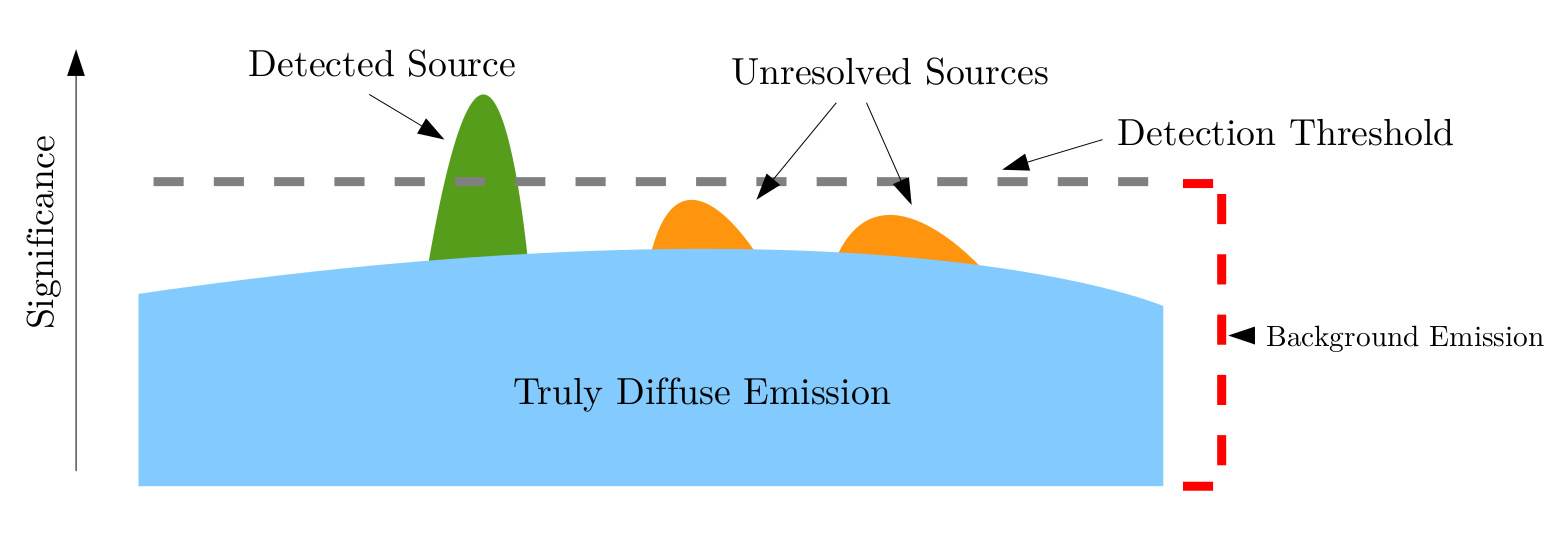
\includegraphics[width=0.5\textwidth]{figures/definitions.png}
  \caption{Illustration for galactic emission definitions.}
\end{wrapfigure}

There is a need in the $\gamma$-ray astronomy community for a reliable method of separating source and background `diffuse' emission in the Milky Way. While such methods have been successfully implemented at lower energies, in high-energy GeV and TeV analysis, these methods are limited by the small number of cosmic rays observed. The challenge thus lies in finding good diffuse estimation methods for this statistics-limited regime.

\subsection{Galactic Emission}

Galactic emission may be regarded as the sum of a number of distinct components. As definitions of these in the literature is non-standardized, we set here conventions for the terminology applied to this work. These definitions are illustrated in Figure 1.

\begin{itemize}
\item{\textbf{Sources} refer to resolvable sources of $\gamma$-rays, above a given instrument detection threshold.}
\item{\textbf{Unresolved sources} are those sources which physically exist but fall below the detection threshold of a given instrument, and so are not distinguished as sources against a background signal.}
\item{\textbf{Truly diffuse galactic emission} refers to the flux contribution from physical processes leading to diffuse cosmic ray emission - at TeV energies, this is dominated by inverse Compton and $\pi^0$ decay while at lower GeV energies bremsstrahlung also contributes significantly.}
\item{\textbf{Galactic background emission} is the Galactic flux contribution which cannot be directly attriubuted to sources. As such, this is considered as the sum of the unresolved and truly diffuse emission contributions. In this work, this Galactic background emission is referred to as `diffuse' emission.}
\end{itemize}

\section{Method}

An algorithm based on significance clipping and convolution with an elongated background filter is introduced. The operation of the algorithm is summarized in the following steps.

\begin{itemize}
\item{\textbf{Initiation step:} Convolution of a counts map with a background kernel to act as an initial background image.}
\item{\textbf{Propagation step:} A significance image is computed from the counts map and background image. From this, an exclusion mask is determined, removing regions above a set significance threshold. These regions are replaced with a background estimation based on the flux around the excluded source. A new background image results from convolution with an elongated background kernel. The step repeats with excluded regions dilated with each iteration for which they fall above the significance threshold.}
\item{\textbf{Termination step:} Once there is no change in the exclusion mask, the propagation step ends and the final background image is returned.}
\end{itemize}

\subsection{Parameters}

The method is specified by six parameters, their values indicated in Table 2.

The significance threshold was set through preliminary studies to understand how to avoid significance-triggering (and hence false source detection) on Poisson up-flucctuations. This was achieved by Poisson-flucctuating a uniform input image, and selecting a significance threshold above that for which false detections were avoided.

\begin{wrapfigure}{l}{0.4\textwidth}
\begin{center}
\begin{tabular}{|c|c|}
\hline
\textbf{Containment/$\%$} & \textbf{Radius/$deg$}\\\hline
68.0 & 0.150 \\\hline
95.0 & 0.867 \\\hline
\end{tabular}
\end{center}
\caption{\textit{Fermi}-LAT PSF Containment representative of the 10-500 GeV energy band \footnotemark.}
\end{wrapfigure}

\footnotetext{The method described by \cite{lw} was used to determine an appropriate representative energy for the range considered.}

The correlation radius and mask dilation radius were chosen to be of the order of the \textit{Fermi}-LAT PSF to optimize for point source detection (see Table 3), while an elongated background kernel was chosen to follow the expected elongated background signal of the Galactic plane. A pixel size of 0.1 degrees offered suitable resolution for Fermi source detection without leading to an excessive computational load during analysis.

\begin{wrapfigure}{r}{0.5\textwidth}
\begin{center}
\begin{tabular}{|c|c|}
\hline
\textbf{Parameter} & \textbf{Value}\\\hline
Significance cut off & 4 $\sigma$\\\hline
Correlation radius & 0.3\degree \\\hline
Mask dilation radius & 0.3\degree \\\hline
Height of background kernel & 0.5\degree \\\hline
Width of background kernel & 10\degree \\\hline
Pixel size & 0.1\degree \\\hline
\end{tabular}
\end{center}
\caption{Values of Separation Algorithm Parameters}
\end{wrapfigure}

\subsection{Region of Interest}

An analysis region of Galactic latitude $-5 < b < 5$ and longitude $-100 < l < 100$ was chosen to encompass the majority of the observed galactic emission. This ensures regions of high source density around the galactic center, with variation in the population distribution at higher longitudes offering a broad base of test cases for the separation method.


\section{Dataset}

The dataset upon which the method is demonstrated was drawn from experimental \textit{Fermi}-LAT observations. Additionally, simulated inputs providing a realistic and well-understood test-base for the method were employed. Both are described here.

\subsection{\textit{Fermi}-LAT}

\textit{Fermi}-LAT data from 5 years of observation was chosen with a well defined 10-500 GeV energy cut as a showcase for the method. This choice was due to a well-understood PSF, good coverage of the Galactic plane, and roughly uniform exposure of the region of interest at these high energies. It should be noted that applications of this method in analyses need not be limited to \textit{Fermi}-LAT data. Image analysis of all high-energy galactic data is the intended use-case.

The available statistics of the energy range in question fall off steeply towards the higher end of the cut. There are thus suitable numbers of events for such an analysis to be undertaken on the data set, but fewer than might be neccessary with a conventional approach with a lower energy dataset. The statistics are outlined in Table 4 and Figure 1.

\begin{wrapfigure}{l}{0.5\textwidth}
  \begin{center}
      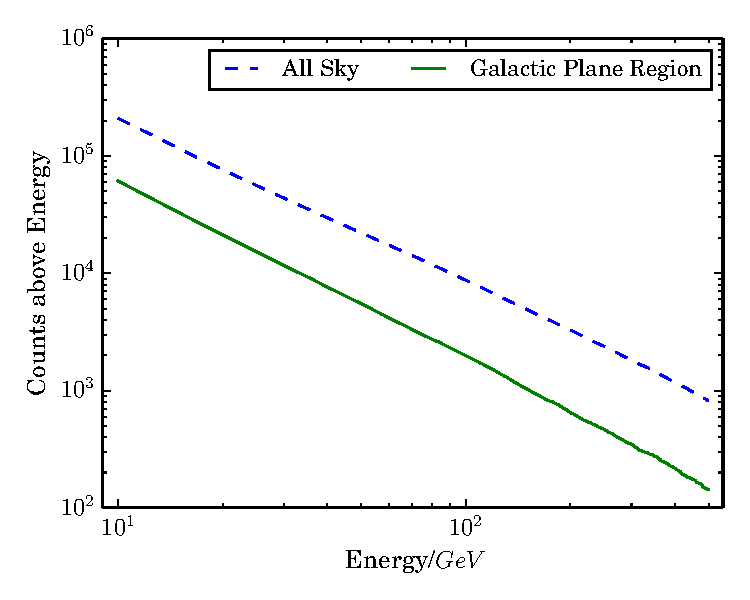
\includegraphics[width=0.5\textwidth]{figures/counts.pdf}
  \caption{Fermi/\textit{LAT} cosmic-ray events detected above energies to illustrate the energy distribution of cosmic-ray detections between 10 and 500 GeV.}
  \end{center}
\end{wrapfigure}

\subsection{Simulation}

The simulated dataset may be split two-fold. In both cases, a well-understood simple source population is added to a known background contribution - in this case, the Fermi diffuse background model \verb|gll_iem_v05_rev1.fit| was taken as a good example to model the morphology of the galactic diffuse emission.

The simulated inputs differ in that one uses a source contribution taken as a PSF-convolved point source image of the entired of the 1FHL catalog above 10 GeV, while the other uses an entirely simulated model set of source populations.

\subsubsection{1FHL Source Population}

In the case where the simulated input took the PSF convolved 1FHL source catalog, the resulting source-only image had a total all-sky flux of $1.60\text{e}^{-7} \text{ph cm}^{-2}\text{s}^{-1}$, of which $2.84\text{e}^{-9} \text{ph cm}^{-2}\text{s}^{-1}$ was contributed by the Galactic plane region of interest.

\subsection{Model Source Populations}

In the case where the source flux contribution was entirely simulated by model galaxies, the inputs were based on the study undertaken in the simulation work of the 1FHL Catalog paper \cite[p.59]{1fhl}, which was largely based on the work in \cite{Strong}. This considered a reference galaxy of a similar source population and distribution to the Milky Way, and two further simulations aiming to provide test cases for source detection with different proportions of bright and faint sources.

In line with \cite{Strong}, it is assumed that the luminosity function of the $\gamma$-ray source population between two limits $L_{\gamma, min}$ and $L_{\gamma, max}$ follows a simple power law of index -1.5 and it is taken that the spatial distribution of pulsars offers representative example of spatial distribution of a galactic $\gamma$-ray source population \cite[p.2]{Strong}. Thus we use a galactocentric $(R, z)$ pulsar distribution model \cite[p.7]{Lorimer} to distribute sources for the $\rho(R)$ radial source density distribution, and an exponential function for the $\rho(z)$ distribution.

\begin{equation}
\rho(R, z) = A\left(\frac{R}{R_{\astrosun}}\right)^{B} \exp\left(-C\left[\frac{R-R_{\astrosun}}{R_{\astrosun}}\right]\right)\exp(-|z|/D)
\end{equation}

$R_{\astrosun}$ is taken as the radial position of the Sun with respect to the galactic center. Standard Monte-Carlo methods are used to sample $\rho(L_{\gamma}, R, z)$ throughout the simulated galaxy and then the resulting distribution is normalized and scaled at $R_{\astrosun}$ to $A = \rho_{\astrosun}$ as the population density of the sun.

In line with the 1FHL study, the radial distribution peaks at 4 kpc - thus $B = 4$ and $C = R_{\astrosun}$. The $\rho(z)$ exponential scale is set to 0.5 kpc (so $D=0.5$).

A reference model is defined with $\rho_{\astrosun} = 3 \text{kpc}^{-3}$ with a minimum $\gamma$ luminosity $L_{\gamma, min} = 10^{34} \text{ph s}^{-1}$ and maximum $\gamma$ luminosity $L_{\gamma, min} = 10^{37} \text{ph s}^{-1}$. Two comparison models - both of higher population densities at the position of the sun and lower luminosity bounds - are also considered. These three models are outlined in Table 3.

\begin{table}
\centering
\resizebox{\textwidth}{!}{
\begin{tabular}{|c|c|c|c|}
\hline
\textbf{Source Model} & \textbf{Population Density at the Sun/$kpc^{-3}$} & \textbf{Minimum Luminosity/$ph s^{-1}$} & \textbf{Maximum Luminosity/$ph s^{-1}$}\\\hline
Reference Simulation & 3 & $10^{34}$ & $10^{37}$\\\hline
Simulation 1 & 10 & $4 \times 10^{33}$ & $4 \times 10^{36}$ \\\hline
Simulation 2 & 30 & $1.5 \times 10^{33}$ & $1.5 \times 10^{36}$ \\\hline
\end{tabular}}
\caption{Parameters for 10 - 500 GeV Galaxy Population Simulations.}
\end{table}

\subsubsection{Simulated Diffuse Contribution}

Before application to the source separation algorithm, the 1FHL and simulated catalogs are added to the integrated Fermi Diffuse background model \verb|gll_iem_v05_rev1.fit| between 10 GeV and 500 GeV to produce source/diffuse test cases. The integral flux of the background model in the galactic plane region contributes an all-sky flux of $4.21\text{e}^{-6} \text{ph cm}^{-2}\text{s}^{-1}$, of which $2.85\text{e}^{-7} \text{ph cm}^{-2}\text{s}^{-1}$ ($6.77\%$) is contributed by the galactic plane region.

\begin{table}
\centering
\resizebox{\textwidth}{!}{
\begin{tabular}{|c|c|c|c|}
\hline
\textbf{Source Model} & \textbf{Total Flux/ph cm$^{-2}$ s$^{-1}$} & \textbf{Flux in Galactic Region/ph cm$^{-2}$ s$^{-1}$} & \textbf{Proportion of Flux in Galactic Region/\%}\\\hline
\textit{Fermi} 1FHL Catalog > 10 GeV & $1.60\text{e}^{-7}$ & $2.84\text{e}^{-9}$ & 1.77\\\hline
Reference Simulation & $9.96\text{e}^{-8}$ & $1.70\text{e}^{-8}$ & 17.1\\\hline
Simulation 1 & $1.93\text{e}^{-7}$ & $1.94\text{e}^{-8}$ & 10.0 \\\hline
Simulation 2 & $1.93\text{e}^{-7}$ & $1.99\text{e}^{-8}$ & 10.3 \\\hline
\end{tabular}}
\caption{Galactic plane fluxes for source population catalogs.}
\end{table}


\section{Results}

The results of this study may be categorized as those relating the the simulated inputs used to understand the algorithm, and those relating to the applicaiton of the separation algorithm to real Fermi-LAT data.

\subsection{Simulation Results}

\begin{wrapfigure}{l}{0.6\textwidth}
\centering
\resizebox{0.6\textwidth}{!}{
\begin{tabular}{|c|c|c|}
\hline
\textbf{Source Model} & \textbf{True Source} & \textbf{Recovered Source}\\
\textbf{(\& Fermi Diffuse Background)} & \textbf{Flux Fraction/\%} & \textbf{Flux Fraction/\%}\\\hline
Fermi 1FHL Catalog > 10 GeV & 0.987 & 1.39\\\hline
Reference Simulation & 5.63 & 3.64\\\hline
Simulation 1 & 6.37 & 2.30\\\hline
Simulation 2 & 6.52 & 1.97\\\hline
\end{tabular}}
\caption{Galaxy Modelling Parameter Values.}
\end{wrapfigure}

\subsubsection{Simulation Results}

\begin{wrapfigure}{c}{\textwidth}
  \begin{center}
      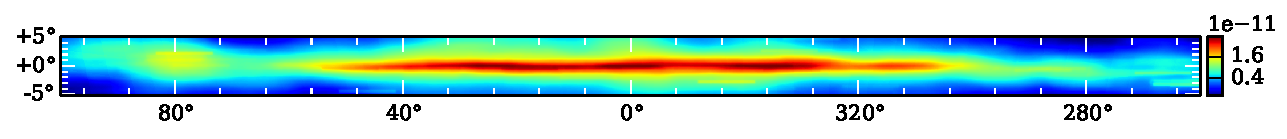
\includegraphics[width=\textwidth]{figures/BG_1FHL.pdf}
  \caption{Background estimation for 1FHL Catalog input image.}
  \end{center}
\end{wrapfigure}

\begin{wrapfigure}{c}{\textwidth}
  \begin{center}
      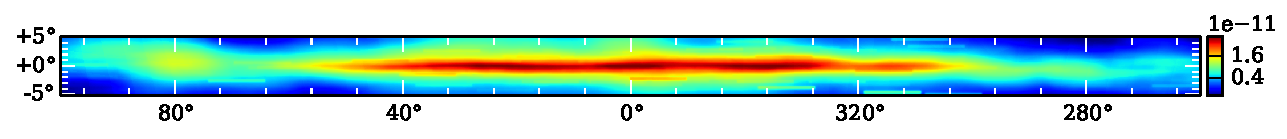
\includegraphics[width=\textwidth]{figures/BG_SIM1.pdf}
  \caption{Background estimation for reference galaxy input image.}
  \end{center}
\end{wrapfigure}

\begin{wrapfigure}{c}{\textwidth}
  \begin{center}
      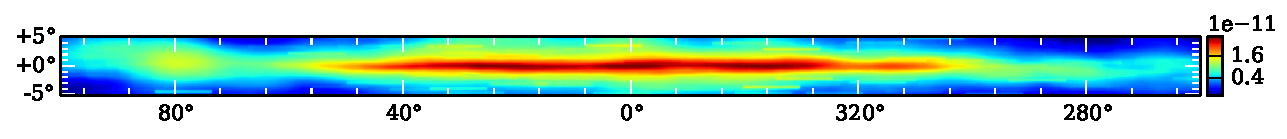
\includegraphics[width=\textwidth]{figures/BG_SIM2.pdf}
  \caption{Background estimation for simulation 2 input image.}
  \end{center}
\end{wrapfigure}

\begin{wrapfigure}{c}{\textwidth}
  \begin{center}
      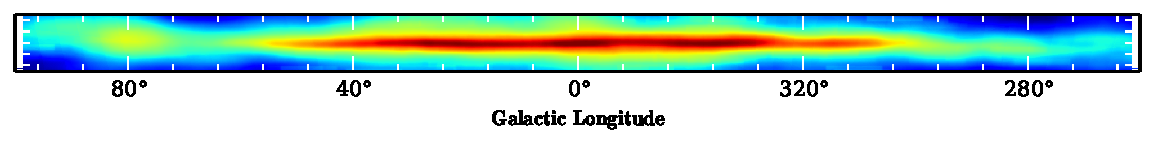
\includegraphics[width=\textwidth]{figures/BG_SIM3.pdf}
  \caption{Background estimation for simulation 3 input image.}
  \end{center}
\end{wrapfigure}


\begin{table}
\centering
\resizebox{\textwidth}{!}{
\begin{tabular}{|c|c|c|c|}
\hline
\textbf{Source Model} & \textbf{Total Flux/ph cm$^{-2}$ s$^{-1}$} & \textbf{Flux in Galactic Region/ph cm$^{-2}$ s$^{-1}$} & \textbf{Proportion of Flux in Galactic Region/\%}\\\hline
\textit{Fermi} 1FHL Catalog > 10 GeV & $4.35\text{e}^{-6}$ & $2.83\text{e}^{-7}$ & 6.52\\\hline
Reference Simulation & $4.30\text{e}^{-6}$ & $2.91\text{e}^{-7}$ & 6.77\\\hline
Simulation 1 & $4.37\text{e}^{-6}$ & $2.97\text{e}^{-7}$ & 6.79 \\\hline
Simulation 2 & $4.39\text{e}^{-6}$ & $2.99\text{e}^{-7}$ & 6.81 \\\hline
\end{tabular}}
\caption{Galactic plane fluxes for separated background images of the input simulation image catalogs.}
\end{table}

\subsubsection{Fermi-LAT Results}

TODO


\begin{table}
\centering
\resizebox{\textwidth}{!}{
\begin{tabular}{|c|c|c|c|}
\hline
\textbf{Source Model} & \textbf{Total Flux/ph cm$^{-2}$ s$^{-1}$} & \textbf{Flux in Galactic Region/ph cm$^{-2}$ s$^{-1}$} & \textbf{Proportion of Flux in Galactic Region/\%}\\\hline
\textit{Fermi}-LAT Observed Data, 10-500 GeV & $1.89\text{e}^{-6}$ & $9.90\text{e}^{-8}$ & 5.24\\\hline
\end{tabular}}
\caption{Galactic plane fluxes for separated background from true Fermi-LAT data.}
\end{table}


\begin{wrapfigure}{c}{\textwidth}
  \begin{center}
      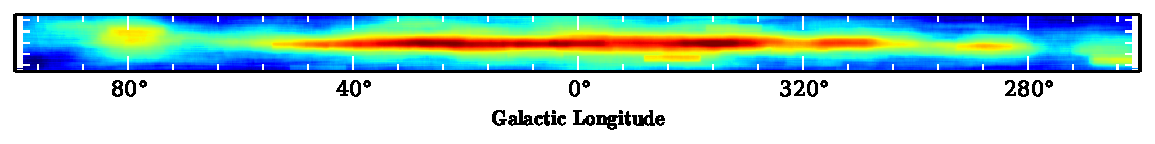
\includegraphics[width=\textwidth]{figures/BG_DATA.pdf}
  \caption{Background estimation for Fermi-LAT Data.}
  \end{center}
\end{wrapfigure}

\begin{wrapfigure}{l}{0.5\textwidth}
  \begin{center}
      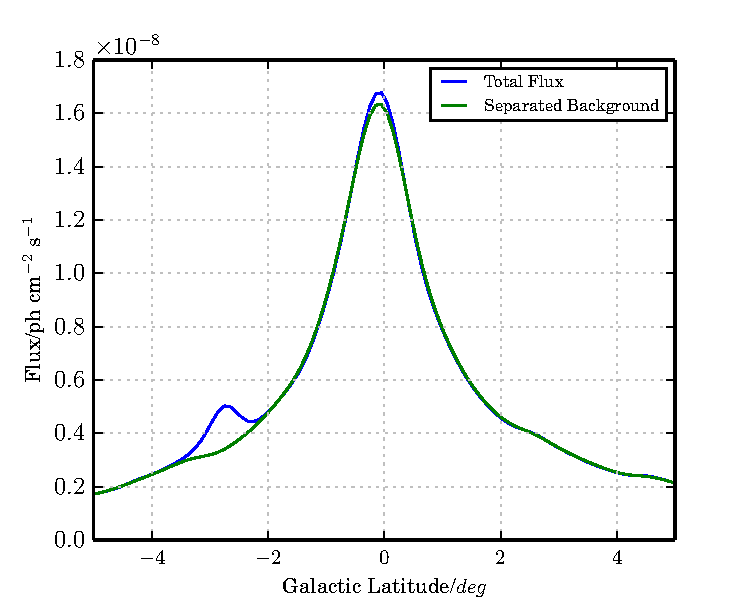
\includegraphics[width=0.5\textwidth]{figures/GLAT.pdf}
  \caption{Galactic latitude profile for initial flux and background model.}
  \end{center}
\end{wrapfigure}

\begin{wrapfigure}{c}{\textwidth}
  \begin{center}
      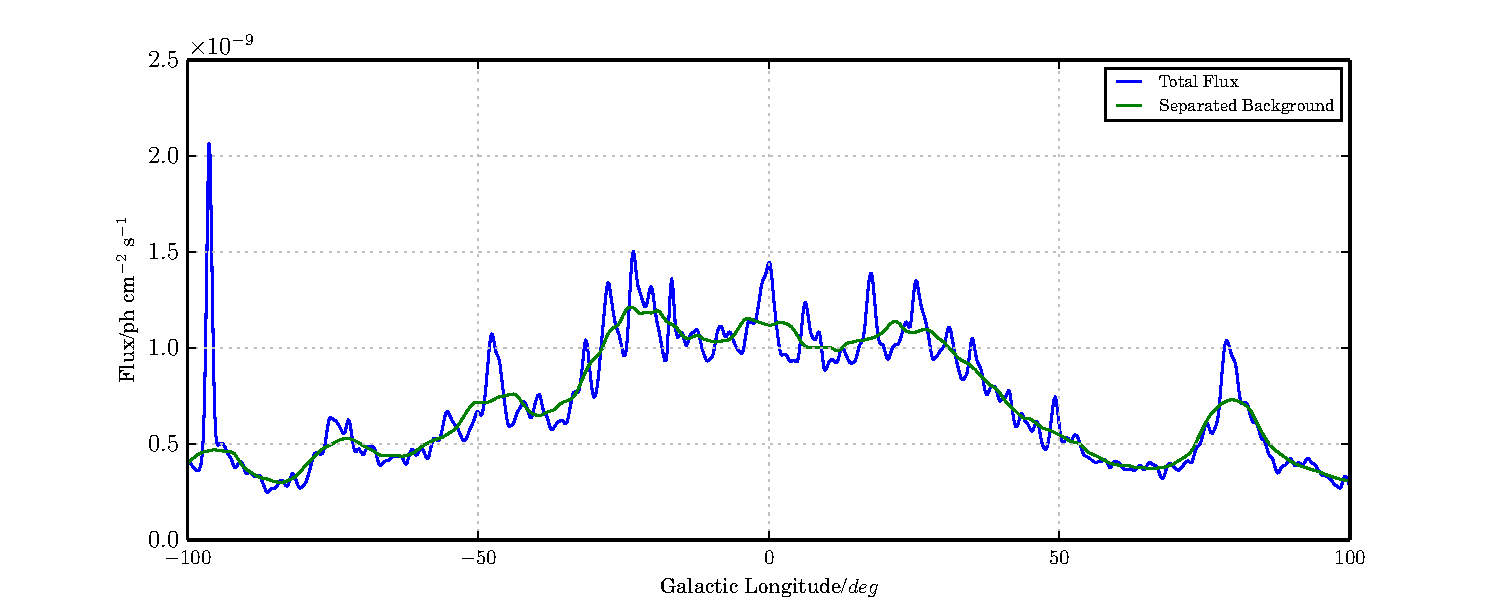
\includegraphics[width=\textwidth]{figures/GLON.pdf}
  \caption{Galactic longitude profile for initial flux and background model.}
  \end{center}
\end{wrapfigure}

\section{Conclusions}

\begin{wrapfigure}{c}{\textwidth}
  \begin{center}
      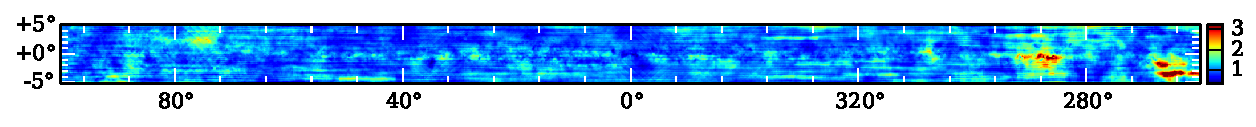
\includegraphics[width=\textwidth]{figures/RATIO.pdf}
  \caption{Ratio of background estimation over fermi diffuse model.}
  \end{center}
\end{wrapfigure}


\section{Summary}
These methods are included in the affiliated astropy open-source package, gammapy \cite{Deil}.

\begin{thebibliography}{99}

\bibliographystyle{plain}
\bibliography{references}


\end{thebibliography}
\end{document}


